\documentclass{article}
\usepackage{tikz}
\usepackage{mathpazo}
\usepackage{xcolor}

\usepackage{verbatim}

\newcounter{row}
\newcounter{col}

\edef\puzzlescale{1.2}
\edef\numrows{4}

\newcommand\setrow[\numrows]{
  \setcounter{col}{1}
  \foreach \n in {#1, #2, #3, #4} {
    \edef\x{\value{col} - 1}
    \edef\y{1 + \numrows - \value{row}}
    \node[anchor=north west,scale=0.75*\puzzlescale] at (\x, \y) {\n};
    \stepcounter{col}
  }
  \stepcounter{row}
}

\newcommand\boldh[3]{
  \edef\y{\numrows-#1}
  \edef\x{#2}
  \edef\z{\x + #3}
  \draw[very thick] (\x, \y) -- (\z, \y);
}

\newcommand\boldv[3]{
  \edef\y{\numrows-#1}
  \edef\x{#2}
  \edef\z{\y - #3}
  \draw[ultra thick] (\x, \y) -- (\x, \z);
}

\definecolor{shadegray}{gray}{0.75}

\newcommand\shadebox[2]{
  \edef\y{\numrows-#1}
  \edef\x{#2}
  \fill[shadegray] (\x, \y) rectangle (\x+1,\y-1);
}

\begin{document}
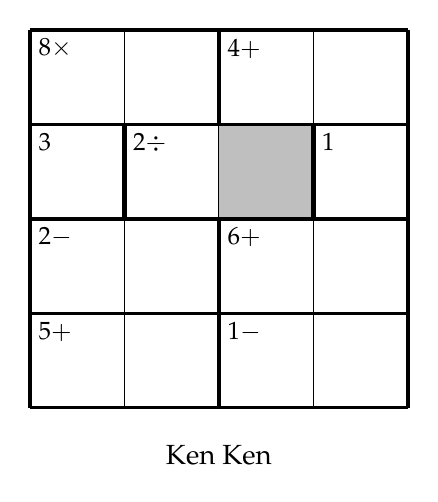
\begin{tikzpicture}[scale=\puzzlescale]

  \begin{scope}

    \shadebox{1}{2}
    
    \draw (0, 0) grid (4, 4);
    \boldh{0}{0}{4}
    \boldh{1}{0}{4}
    \boldh{2}{0}{4}
    \boldh{3}{0}{4}
    \boldh{4}{0}{4}
    \boldv{0}{0}{4}
    \boldv{1}{3}{1}
    \boldv{1}{1}{1}
    \boldv{0}{2}{1}
    \boldv{2}{2}{2}
    \boldv{0}{4}{4}

    \setcounter{row}{1}
    \setrow {$8\times$} {} {$4+$} {}
    \setrow {$3$} {$2\div$} {} {$1$}
    \setrow {$2-$} {} {$6+$} {}
    \setrow {$5+$} {} {$1-$} {}
    
    \node[anchor=center] at (0.5*\numrows, -0.5) {Ken Ken};
  \end{scope}

\end{tikzpicture}

\end{document}
